\documentclass{article}
\usepackage[margin=1.25in]{geometry}
\usepackage{fancyhdr}
\usepackage{graphicx}
\usepackage{vhistory}
\usepackage[parfill]{parskip}
\graphicspath{{../Images/}}

\renewcommand{\baselinestretch}{1.5}

% Set fancy looking header/footer and move page number to the right
\pagestyle{fancy}
\fancyhead{}
\fancyfoot{}
\fancyfoot[R]{\thepage}

\patchcmd{\section}{-3.5ex \@plus -1ex \@minus -.2ex}{-3.5ex \@plus -1ex \@minus -.2ex\setlength{\leftskip}{0cm}}{}{}
\patchcmd{\subsection}{-3.25ex\@plus -1ex \@minus -.2ex}{3.25ex\@plus -1ex \@minus -.2ex\setlength{\leftskip}{1cm}}{}{}
\patchcmd{\subsubsection}{1.5ex \@plus .2ex}{1.5ex \@plus .2ex\setlength{\leftskip}{2cm}}{}{}

\begin{document}
    \pagenumbering{gobble}
    \begin{titlepage}
    \begin{center}
        \vspace*{1cm}

        \Huge
        \textbf{User's Guide for Cloud Backup}

        \vspace{.5cm}
        \LARGE
        Captain CyBeard: Neil Before Us

        \vspace{1cm}

        \textbf{Ryan Breitenfeldt \textbar\ Noah Farris\\ Trevor Surface \textbar\ Kyle Thomas}

        \vspace{.2cm}
        \Large
        May 4, 2020

        \vspace{2cm}
        
\includegraphics[scale=1]{logo}

        \vfill

        Washington State University Tri-Cities\\
        CptS 423 Software Design Project 2

    \end{center}
\end{titlepage}




    \tableofcontents
    \newpage
    \listoffigures


    \newpage
    \begin{versionhistory}
        \vhEntry{3.0}{05.03.2020}{KT}{Updated requirements to reflect the application and customer changes.}
        \vhEntry{2.2}{12.07.2019}{KT}{Added in Dr. Corrigan's corrections}
        \vhEntry{2.1}{12.04.2019}{TS}{Provided more grammatical checking along with a Reference Recommendation}
        \vhEntry{2.0}{12.04.2019}{KT}{Added priority section \& final edits}
        \vhEntry{1.2}{12.03.2019}{KT}{Grammar edits and wording}
        \vhEntry{1.1}{11.16.2019}{NF}{Grammar edits and wording}
        \vhEntry{1.0}{11.15.2019}{RB NF TS KT}{First Final Doc}
        \vhEntry{0.9}{11.14.2019}{KT}{Spelling \& grammar edits}
        \vhEntry{0.8}{11.12.2019}{TS}{Added more components to subsections for length}
        \vhEntry{0.7}{10.29.2019}{NF}{Edits to whole doc}
        \vhEntry{0.6}{10.29.2019}{KT}{Edits}
        \vhEntry{0.5}{10.28.2019}{NF}{Background}
        \vhEntry{0.4}{10.28.2019}{RB}{Introduction}
        \vhEntry{0.3}{10.15.2019}{TS}{Completed Overview}
        \vhEntry{0.2}{10.10.2019}{RB NF TS KT}{Filled in Environment \& Operation sections}
        \vhEntry{0.1}{09.27.2019}{KT}{Document Creation}
    \end{versionhistory}
    \newpage


    \pagenumbering{arabic}
    \section{Introduction}
    This requirements specification document will go over the requirements for the Virtual Machine file Downloader for Cypherpath's Resiliency Platform \cite{cypherpath} that was outlined in the
    \texttt{Project Plan} \cite{projectplan}. This \textit{Downloader} application will allow users to transfer files directly from various cloud platforms into the Resiliency Platform
    created by Cypherpath that gives their customers cyber resiliency.
    The document will cover how the application will provide a solution for users to easily upload their Virtual Machine files to the Resiliency Platform.
    Along with covering the solution, the requirements specification will also provide details on how users will interact with the application through a web interface.
    This document will be understood and agreed upon by both the customer (Cypherpath) and the software development team (Captain CyBeard).

    Subsequent sections will include background information on Cypherpath and their Resiliency Platform, followed by a high level overview of the application. After this, the document will get into the
    details of the application such as the environment the application will execute in, and how the application will be operated by users and web administrators.

	  The Cypherpath Resiliency Platform tool is a product that provides their customers the ability to upload pre-existing virtual machines, network configurations and more, into 
    a self-contained digital environment. This enables their customers to quickly recover from events such as ransomware attacks or human errors. Right now, customers have to manually download their virtual disk images from
    the various cloud platforms they are hosted on, and then upload those to the Resiliency Platform. Cypherpath would like to have a web application that will enable users to have their virtual disk images go
    directly from the cloud platform into the Resiliency Platform, cutting out the multi-step process of downloading and then uploading large virtual disk images.
	
    \section{Background}
    Cypherpath's Resiliency Platform started out as a platform where the U.S. Military could emulate the networks of countries and simulate cyber attacks between the countries in order to
    learn about the strength and weaknesses of the countries simulated. After proving its usefulness in this market, Cypherpath entered the commercial market and provides its platform as a service to
    companies and local governments alike to provide resiliency to these entity's network infrastructures. Resiliency in the cyber sense means that systems and networks are secure, recoverable and
    continuous. Customers of Cypherpath enjoy a readiness of their technological resources, and can rapidly adjust and adapt those resources when failures, damages or attacks occur in order to keep their business running smoothly.

    This project will become a component of the Resiliency Platform by enabling Cypherpath's customers to more easily migrate their virtual assets into the platform. Currently customers have to download
    their virtual assets onto their local machine and then upload them into the Resiliency Platform. This project will simplify this process by having the Resiliency Platform download the virtual asset directly
    into its infrastructure. The software development team will not be integrating the application with the Resiliency Platform. The product delivered to Cypherpath will be a standalone web application that downloads
    digital assets from various cloud platforms. Upon completion of the project, Cypherpath will integrate the web application into their Resiliency Platform by changing the user interface and theme of the application to match
    theirs. They only need the backend Python-Django part of the application.

	
    \section{Overview}
    The purpose of this application is to allow users to download virtual disk images from online cloud platforms, to the Resiliency Platform (the application delivered will only download the files to local storage).
    Currently, Cypherpath customers manually visit each of their cloud platforms and download their files, then upload them into the Resiliency Platform. This application will act as middleware and direct the download
    into the Resiliency Platform.
    The application itself will operate as a web server using Python3.8+ \cite{python} and Django2.2+ \cite{django}. Users will start the application by navigating to the URL pointing to the application.
    Once at the main page the user will select a cloud platform from a pull down menu and then be directed to authenticate to the selected platform. After authentication, the application will use the API of the cloud
    platform and show the user their files stored on the platform.
    The user will be able to navigate their directory structure and select which files and folders to load into the platform (again, during development the application will download the files to local storage instead
    of interacting with the Resiliency Platform).

    The application will be written with Python3.8+ and Django2.2+, including the requests libraries for API calls, Authentication libraries like SAML
    and standard libraries. To install the application, Cypherpath will integrate the Django web application into their environment along with installing (if not installed already)
    the libraries for interacting with the external cloud platforms and authentication API's. Users of the application will not need to install any software since most operating systems come
    with a web browser which will interact with the application on the user's end.


    \section{Environment}
    This section will describe the environment the application will reside in. This will include the web application, authentication API's, cloud storage API's and the local storage
    of the machine running the application. During development this will be the users machine, but Cypherpath will be using their storage scheme for production.
	
    \begin{figure}[h]
    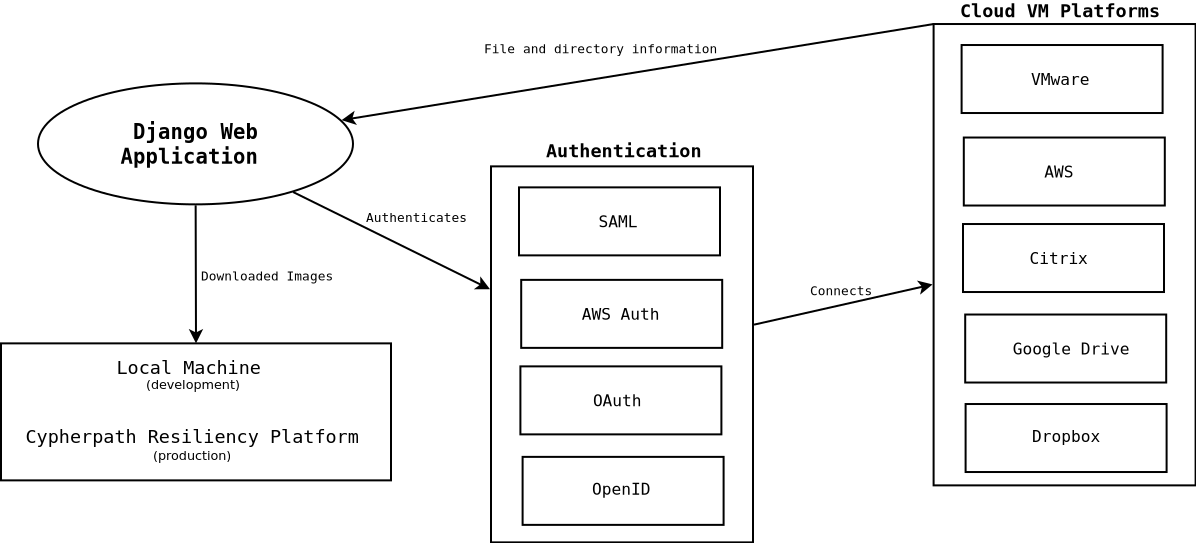
\includegraphics[scale=.4]{downloader_env}
        \caption{A visual representation of the applications environment.}
    \end{figure}


        \subsection{Web Application}
        The web server for the application during development will be Django's built in development server and when the project is completed, Cypherpath will integrate
        the web application into their existing ecosystem using their webserver. The Django application will host the functionality of the application, including HTML templates for the 
        web pages, where users provide Virtual Machine URLs and browse their directories. Additionally, the Django framework will allow the usage of Python classes that will enable the 
        back-end operation of the application.

        
        \subsection{Authentication API's}
        The application will authenticate to the cloud platforms with various authentication methods and API's. The application will support
        the authentication for various platforms. Some will use OAuth2 or variations of it and redirect to the cloud provider's authentication, others will use a custom
        login page to obtain the user's credentials (like AWS). The application will be designed in a modular fashion so that more authentication methods can be easily added later.


        \subsection{Cloud Storage API's}
        Once the application is authenticated to a cloud storage platform it will gather the list of files on the platform for showing to the user and allowing them to select
        which of their files they would like to download. The application will support interacting with Amazon Web Services \cite{aws}, Google Drive and Dropbox. The API's
        that are necessary for the communication, will request the directory structure of their cloud storage and provide it to the user so they can select which files
        from the cloud platform, they would like to download. Like the authentication modules, the modules
        for interacting with the cloud API's will need to be designed so that adding support for other cloud platforms will be possible.


        \subsection{Local Storage}
        Once the user has selected which files to download from their cloud platform, the application will download those
        files to the user's local storage. The application will download all of the user's selected files from the cloud platform to their local storage.
        The local storage location will be determined by the web server, the application will download the files from the cloud platform to a location specified by the application backend. Nothing else 
        needs to be done with the files because after the application is finished and Cypherpath has integrated the web application into 
        their platform, they will direct the downloads where they need them.


    \section{Operation}
    In the following sections the operation of the application will be described, including starting the application
    (invocation) from the user's perspective and the web server administrator, the commands the application uses and finally, how users and administrators will terminate the application.

        \subsection{Invocation}
        During development the application will be started using Django's built-in webserver and
        the user will not need to be authenticated to use the application. To invoke the application the user will simply enter the URL for the application (such as http://localhost:8080).
        They will then be presented with the main screen of the application. The screen will have a single pull down menu for a user to select a cloud platform. Additionally 
        a submit button will be provided for them to continue to step through the application. 

        To start the development server, the developer/mock web administrator will use the following commands in the Django project directory containing the \textit{manage.py} file.
        \begin{verbatim}
        $ python manage.py migrate  # only necessary to run the first time
        $ python manage.py runserver
        \end{verbatim}

        The user will now be able to use their web browser to visit the main page.

        The user interface and invocation of the application are simple. Later when Cypherpath integrates the application into their Resiliency Platform, invocation by the user will be from within Cypherpath's
        platform. Cypherpath does not have preferences on the user interface since they will be adding their own style, layout, themes, etc.\ to the user interface. The server side of the application will be invoked
        from Cypherpath's web server that serves their platform.

        \subsection{User Actions}
        This section covers how the user will interact with the application and how entering the application, displaying the file structure, downloading virtual disk images and error catching 
        will be implemented.

            \subsubsection{Select Platform}
            On the main page of the application the user will be presented with a pull down menu where they will select a cloud platform. The menu will be centrally located with a design to
            help users clearly see where to select the platform. Once a platform is selected and submitted the application will invoke the authentication methods for that cloud platform. This may be redirecting the user
            the cloud platform's authentication or prompting the user for their credentials and passing those directly to the cloud platform.
            Once authenticated the application will present the user with their files and folders that are on that platform.
            
            \subsubsection{Display File Structure and Download Selected Files}
            Once the user has selected a cloud platform and is authenticated, they will be presented with their files that are stored on that platform. They can use this information to verify all files were retrieved
            from the cloud once downloaded and select which
            files to download. After selecting the files the user wants, they will click the download button, which initiates the download of their selected files from the cloud platform.
            This will redirect the user to a page showing them just the files that they selected. During development, the application server will download the files to a location on server's local drive.
            When Cypherpath assimilates the application into their platform they will direct the download where they need it. This will be accomplished by Cypherpath changing the location that the application server
            stores the downloads.

            These pages that present the user with their files and downloads will also contain a ``start over'' button, which will bring them back to the main page.

            \subsubsection{Error Catching}
            Errors will be detected through the various aspects of the program. If there are not any cloud platforms install on the application, the pull down menu will gracefully display so. If the user does not
            provide valid credentials to the external cloud platform they will be prompted to re-enter their credentials.
            The application will not enforce a limit on the number of authentication attempts the user can make, however the external authentication API or the cloud platform may have limits that it will enforce.
            Additionally if the download fails and the web browser's download manager is unable to recover or restart the download then the user will have to press the download button again assuming they haven't left
            the page.

        \subsection{Termination}
        Since the user is not authenticated to the web application, to terminate their interaction with the application they will simply close the browser tab or window that has the
        application open. Use of the authentication token will be deleted as well per use, there will be no cookies to remember users every time they log into the accounts. After termination
        of the application the user will have to go through the same steps when they invoke the application since sessions and states are not remembered by the application.

        During development the Django Web Server that is used will be terminated by the developer entering \textit{ctrl + c} on their keyboard to end the process. Once Cypherpath has integrated the application into
        their ecosystem they will terminate the web application their way.

    \section{Priority of Cloud Platforms}
    Cypherpath has expressed that Amazon Web Services is their priority to have supported with the application. After those modules are working, Captain Cybeard will then add support
    for Google Drive, Dropbox, and Citrix in that order of priority. The requirement is that at least Amazon Web Services be supported.

    At first, VMware's platforms were the priority, however with the acquisition of Cypherpath they no longer prioritized VMware since setting up a VSphere cloud instance to support was no longer feasible.
    
    
    \newpage
    \begin{thebibliography}{6}
    \bibitem{projectplan}
    Ryan Breitenfeldt, Noah Farris, Trevor Surface, Kyle Thomas.
    \textit{Project Plan}.
    [\textit{Project Plan for Downloader Application}] 2019.

    \bibitem{cypherpath}
    Cypherpath.com. (2019). Cypherpath, Inc. [online] Available at: https://www.cypherpath.com/ [Accessed 21 Oct. 2019].

    \bibitem{aws}
    Amazon Web Services, Inc. (2019). Amazon Web Services (AWS) - Cloud Computing Services. [online] Available at: https://aws.amazon.com/ [Accessed 10 Oct. 2019].

    \bibitem{python}
    Python.org. (2019). Welcome to Python.org. [online] Available at: https://www.python.org/ [Accessed 6 Nov. 2019].

    \bibitem{django}
    Djangoproject.com. (2019). The Web framework for perfectionists with deadlines \textbar\ Django. [online] Available at: https://www.djangoproject.com/ [Accessed 6 Nov. 2019].
    \end{thebibliography}

\end{document}
